
\paragraph{Displacement on $S_1$ is small.}
Note that (1) the adjacent disks in a perfect snowflake cannot be adjacent in a given perturbed snowflake of $S_1$ and (2) $S_1 \subseteq S_i$ for any $i \in \bbN$ because every contact is encoded in the tree.  
Given a snowflake in arbirary position with $i$ nodes per arm; the edge length of each segment is $2r$ except the edges having node $v_0$, these edges are length $2r+ \zeta$.  
The arm has a length of at most $2ri+\zeta$.
Figure \ref{fig:LineSegmentDelta.pdf} shows an arm of a tree in arbitrary position corresponds to a compression and shift of vertices.  
The arm realized in arbitrary position in Figure \ref{fig:LineSegmentDelta.pdf} is analgous to a tree realized in arbitrary position where vertices are in a different position than canonical.  
Our goal is to show that for any $\epsilon >0$ and $x >0$, the position of the center $v$ of any disk in the disk arrangement in any arbitrary realization corresponding to $T_\epsilon$ has a small displacement, i.e. $v$ is found in an open ball referenced at the canonical position of $v$, $v_c$: $$v \in b_{\psi_1}(v_c).$$ 
The definition of $\psi_1$ is shown later on.

\begin{minipage}{\linewidth}
\begin{center}
\includegraphics[width=.95\columnwidth]{graphics/LineSegmentDelta.pdf}
\captionof{figure}{The polyline at the bottom represents a snowflake arm in canonical position.  The polyline above represents a snowflake arm in non-canonical position.}\label{fig:LineSegmentDelta.pdf}
\end{center}
\end{minipage}
 
In a perfect snowflake of $S_1$ the six disks around the central disk kiss.  
The angle formed from the center of the central disk to the centers of any two adjacent disks is $\frac{\pi}{3}$.  
The side lengths of the equalateral triangle formed by the centers of three adjacent disks, one of which is the central disk, is $2\epsilon$.  
For a perturbed $S_1$ the the central disk is weighted $\epsilon+ \zeta$.  
This can yield a change of angular displacement $\frac{\pi}{3}$ to $\frac{\pi}{3} \pm 2\chi$.  
To find the bounds of how large or small $\chi$ can be, we show a trigonometric relation of the half angle of the triangle corresponding to three adjacent disks (See Figure \ref{fig:part1ch4.pdf}).

\begin{minipage}{\linewidth}
\begin{center}
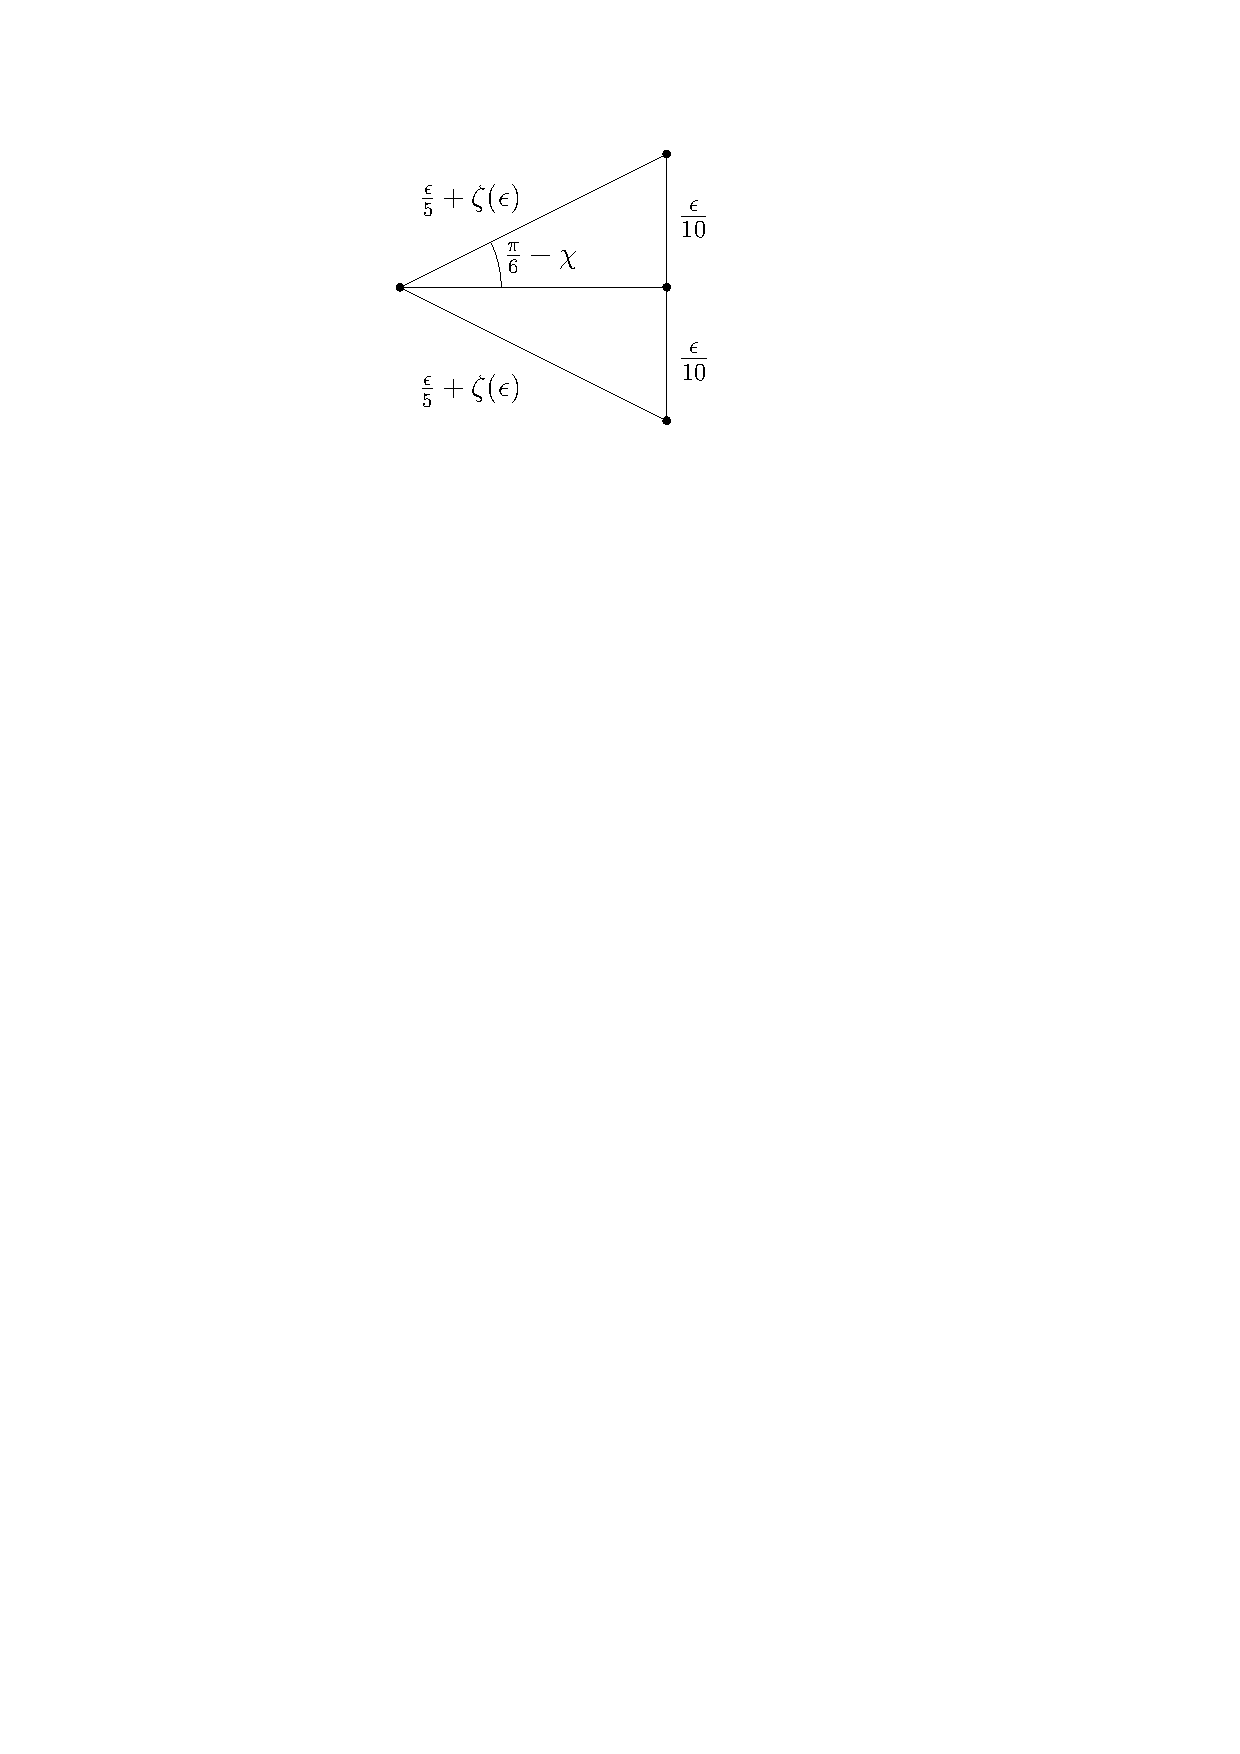
\includegraphics[width=.20\columnwidth]{graphics/part1ch4.pdf}
\captionof{figure}{This figure depicts a triangle corresponding to the center of the central disk and two adjacent disks.}\label{fig:part1ch4.pdf}
\end{center}
\end{minipage}

\begin{eqnarray*}
\sin \lr{\frac{\pi}{6} - \chi} &=& \frac{\epsilon}{2\epsilon+\zeta}\\
\frac{1}{2}\cos \chi = \sin \frac{\pi}{6} \cos \chi &=& \frac{\epsilon}{2\epsilon+\zeta} + \cos \frac{\pi}{6} \sin \chi = \frac{\epsilon}{2\epsilon+\zeta} +\frac{\sqrt{3}}{2} \sin \chi \\
&\Rightarrow&\\
\frac{\epsilon}{2\epsilon+\zeta} + \frac{\sqrt{3}}{2} \lr{ \chi - \frac{\chi^3}{6}} &\leq& \frac{\epsilon}{2\epsilon+\zeta} + \frac{\sqrt{3}}{2} \sin \chi =\frac{1}{2} \cos \chi\\
&\Rightarrow&\\
\frac{\sqrt{3}}{2} \lr{ \chi - \frac{\chi^3}{6}}&\leq& \frac{1}{2}-\frac{\epsilon}{2\epsilon+\zeta}  \qquad \text{if }\chi < 1 \\
\frac{5\sqrt{3}}{12} \chi &\leq&\frac{2\epsilon + \zeta - 2\epsilon}{2 ( 2\epsilon + \zeta)} \\
\chi &\leq& \frac{6}{5 \sqrt{3}}\frac{\zeta}{ 2\epsilon + \zeta} 
\end{eqnarray*}
For any $\epsilon > 0$, the bounds for angular displacement formed at the center of the central disk and two adjacent disks is:
$$ \frac{\pi}{3} - \frac{12 \zeta}{5\sqrt{3}} \leq \frac{\pi}{3} - 2 \chi = 2\chi_\text{min} \leq 2\chi \leq 2\chi_\text{max} = \frac{\pi}{3} + 2 \chi \leq \frac{\pi}{3} + \frac{12 \zeta}{5\sqrt{3}}$$
This shows the bounds of the angular displacement around the central disk.  
To translate this to a coordinate displacement of the centers of the disks around the central disk, we compute a the radius of the ball of radius $\psi$ in which the centers may lie. 
$$\psi = \lr{2 r + \zeta} \sin \chi$$
Using the Maclaurin series of $\sin \chi$:
$$
\begin{array}{rcl}
\psi_i &=& \lr{2 \epsilon + \zeta} \sin \chi\\
&\leq& \lr{2 \epsilon + \zeta} \frac{6}{5 \sqrt{3}}\frac{\zeta}{ 2\epsilon+ \zeta} \\
&=& \frac{6\zeta}{5 \sqrt{3}}
\end{array}
$$
The coordinates of the centers of the disks are close to cannonical position following the angular displacement argument above.  
That is, if $u$ is a center of a disk in a realization to $T_\epsilon$, $u$ lies in a ball $b_{\psi_1}\lr{u_c}$ where $u_c$ is the cannonical position of the $u$.  

\paragraph{Displacement on the arms is small.}
Without loss of generality, consider a path of vertices along a distinct arm, petiole, or leaf $\lr{v_1, v_2, \ldots, v_n}$.  
In the case that there are two paths attached to each vertex, four different angles about the vertex are formed.  
For the $\ith$ vertex, the counter clockwise order of the angles are $\lr{\alpha_{i+1}, \gamma_i, \delta_i, \beta_{i+1}}$ (See Figure \ref{fig:ch4Paralellogram.pdf} for reference).  
We want to establish an angular relationship between two consecutive vertices in a path.
\begin{lem}\label{lem:hingedPolygon27}
Let $\lr{a,b,c,d}$ be a polygonal path in the plane such that the unit disks centered at $a$, $b$, $c$, and $d$ are interior-disjoint.  Then the sum of the two angles on each side at the two interioir vertices is greater than $\pi$. Then the sum of the two angles on each side at the two interior vertices is greater than $\pi$.
\end{lem}
\begin{proof}
Without loss of generality, consider the two angles on the left side  at the two interioir vertices, $\angle abc$ and $\angle bcd$.  We have $\vlr{ab} = \vlr{bc} = \vlr{cd} = 2$, since we have a disk arrangement of unit disks.  If $\lr{a,b,c,d}$ is a rhombus, then $\vlr{ad}=2$ and $\angle abc + \angle bcd = \pi$.  Hence $\vlr{ad}>2$ implies $\angle abc + \angle bcd > \pi$. 
\end{proof}

\begin{minipage}{\linewidth}
\begin{center}
\includegraphics[width=.75\columnwidth]{graphics/lemmaHingedPolygon2.pdf}
\captionof{figure}{(a)Four disks centered along a polygonal path $\lr{a,b,c,d}$ in various drawings.}\label{fig:lemmaHingedPolygon2.pdf}
\end{center}
\end{minipage}

We can now say that for any two consecutive vertices $\lr{v_i, v_{i+1}}$ along a path, the following angular relationship from Lemma \ref{lem:hingedPolygon27}:
$$ 
\begin{array}{rcl}
\pi &<& \alpha_i + \gamma_i \\
\pi &<& \beta_i + \delta_i
\end{array}
$$
This result shows that a perturbed snowflake removes the issue of having unintended constacts that do not reflect a give tree's edge relations that a perfect snowflake has.  

In Figure \ref{fig:ch4Paralellogram.pdf}(a), we have a parallelogram with four unit disks centered, one on each of the vertices of the parallelogram.  
If $\alpha_i + \gamma_{i+1} < \pi$, One of the disks will overlap with another.  
For any arbitrary realization of a perturbed snowflake, any two consecutive angles formed between two adjacent vertices along a path must satisfy the following constraint $$\alpha_i + \gamma_{i+1} \geq \pi.$$

\begin{minipage}{\linewidth}
\begin{center}
\includegraphics[width=.75\columnwidth]{graphics/ch4Paralellogram.pdf}
\captionof{figure}{(a)Four disks of the snowflake shown where the top two disks can either be leaves off petioles or off the arms. (b)An arm depicted at the $\ith$ and $(i+1)^\text{st}$ vertex.}\label{fig:ch4Paralellogram.pdf}
\end{center}
\end{minipage}

To show that the angluar displacement along the arm is small, we extend the angular argument on the perturbed $S_1$ and by induction, show that it is small for all $i$.  
Denote the angles on the concave side of the $\ith$ vertex as $\alpha_i$ and $\beta_i$ and the convex side of the $(i+1)^\text{st}$ vertex as $\gamma_i$ and $\delta_i$ respectively (see Figure \ref{fig:ch4Paralellogram.pdf}(b) for reference). 
For any vertex, the sum of angles about the vertex is $2 \pi$, e.g.:
$$\gamma_i + \delta_i + \alpha_{i+1} + \beta_{i+1} = 2 \pi$$ 

Suppose we numbered the disks about the central disk 1 through 6.  
Without loss of generality, the angles $\alpha_0$ and $\beta_0$ correspond to the angles formed between the central angle, disks $i$ and $i+1$ and disks $i+1$ and $i+2$ respectively, for $i = 1,2,3$.  
The bounds for $\alpha_0$ and $\beta_0$ are the same as $2\chi$ in the earlier argument, i.e.:
$$
\begin{array}{rcccl}
\frac{\pi}{3} - \frac{12 \zeta}{5\sqrt{3}} &\leq& \alpha_0 &\leq& \frac{\pi}{3} + \frac{12 \zeta}{5\sqrt{3}}\\
\frac{\pi}{3} - \frac{12 \zeta}{5\sqrt{3}} &\leq& \beta_0 &\leq& \frac{\pi}{3} + \frac{12 \zeta}{5\sqrt{3}}\\
\end{array}
$$

For $i=0$ we know that $\alpha_0 + \beta_0 \leq \frac{2\pi}{3} + \frac{24 \zeta}{5\sqrt{3}}.$
For the inductive step, suppose the following:
$$
\begin{array}{rcl}
\alpha_i +\beta_i &\leq& \frac{2 \pi}{3} + \frac{24 \zeta}{5\sqrt3}\\
\pi &\leq& \alpha_i + \gamma_i \\
\pi &\leq& \beta_i + \delta_i
\end{array}
$$ 
% State up-front that this is the inequality that you prove by induction. This inequality is true in the base case, i=0, and then you show the induction step

$$
\begin{array}{rcl}
\alpha_i +\beta_i &\leq& \frac{2 \pi}{3} + \frac{24 \zeta}{5\sqrt3}\\
\pi &\leq& \alpha_i + \gamma_i \\
\pi &\leq& \beta_i + \delta_i
\end{array}
$$

Together, we have the following result:
\begin{eqnarray*}
2\pi &=& \alpha_i + \gamma_i + \beta_i + \delta_i\\
 &=& \alpha_i + \gamma_i + \lr{2\pi - \alpha_{i+1} - \beta_{i+1}}\\
 &\iff&\\
\alpha_{i+1} + \beta_{i+1}&=&\alpha_i + \gamma_i \\
&\leq& \frac{2\pi}{3} + \frac{24\zeta}{5\sqrt{3}}\\
\end{eqnarray*}
And so the error bounds on $\frac{\pi}{3}+2\chi$ hold in general for $\alpha_i$ and $\beta_i$ for all $i$.  
$$\alpha_i + \beta_i \leq \frac{2\pi}{3} + \frac{24\zeta}{5\sqrt{3}}$$

\begin{minipage}{\linewidth}
\begin{center}
\includegraphics[width=.75\columnwidth]{graphics/psiSegmentChange.pdf}
\captionof{figure}{This figure illustrates the change of position of the centers of a disk in an arbitrary positin and in a straight, canoncial position. }\label{fig:psiSegmentChange.pdf}
\end{center}
\end{minipage}

A perturbed snowflake is a realization of some tree $T_\epsilon$.  
For the $\jth$ vertex along some path from $v_0$ to $v_j$ (see Figure \ref{fig:psiSegmentChange.pdf} for reference), we can compute the bound of coordinate displacement $\psi_i$ of the disk corresponding to $v_j$ using our inductive argument on the angular displacement above.  
Without loss of generality, to translate the $\jth$ coordinate displacement, we compute the radius of the ball of radius $\psi_i$ in which the $\jth$ center may lie. 
$$\psi_j = \lr{j \epsilon + \zeta} \sin \chi$$
Using the Maclaurin series of $\sin \chi$:
$$
\begin{array}{rcl}
\psi_j &=& \lr{j \epsilon + \zeta} \sin \chi\\
&\leq& \lr{j \epsilon + \zeta} \frac{6}{5 \sqrt{3}}\frac{\zeta}{ 2\epsilon + \zeta} \\
&=& \frac{6}{5}\frac{\zeta\lr{j \epsilon + \zeta}}{2 \epsilon + \zeta}\\
\end{array}
$$
We need to find $\zeta$ such that:
$$ 
\begin{array}{rcl}
\frac{6}{5}\frac{\zeta\lr{j \epsilon + \zeta}}{2 \epsilon + \zeta} &\leq& \epsilon\\
6j\epsilon \zeta + 6 \zeta^2  &\leq& 10 \epsilon^2 + 5 \epsilon \zeta\\
\frac{(6j-5) \epsilon \zeta}{2}\leq (6j-5)\epsilon \zeta + 6 \zeta^2  &\leq& 10 \epsilon^2 \\
\zeta&\leq& \frac{20\epsilon}{6j-5}\\
&\leq& \frac{10 \epsilon}{3j}
\end{array}
$$
Since $j\leq i$, let $\zeta= 2i\epsilon$ and we can bound $\psi_i$:
$$
\begin{array}{rcl}
\psi_i &=& \frac{6}{5}\frac{\zeta\lr{j \epsilon + \zeta}}{2 \epsilon + \zeta}\\
&=& \frac{12 i\epsilon \lr{ \epsilon + 2i\epsilon}}{5\lr{2 \epsilon + 2i\epsilon}}\\
&=&\frac{12 i \epsilon^2 + 24 i^2 \epsilon }{10 (i+1) \epsilon}\\
&=&\frac{12i\epsilon + 24i^2}{10(i+1)}\\
&\leq& \frac{36(i+1)^2 \epsilon}{10(i+1)}\\
&\leq& 4(i+1)\epsilon
\end{array}
$$
We now relax $\psi_i = 4(i+1)\epsilon$. Finally we can say that the displacement of the $\jth$ center denoted as $v^j$ of a disk lies in the ball $b_{\psi_i}(v^j_c)$ around the canonical position $v_c^j$.

\paragraph{Displacement on the petioles is small.}
Note that the petioles have the same geometric structure as the arms; the exception is the number of leaves on each side of the petioles. 
Since we've shown that the geometric shape in arbirary position is already close to canonical position for any $\epsilon>0$, the same argument applies here for the petioles.

We have shown the displacements of all components of the perturbed snowflake are small for any $\epsilon > 0$.  
This shows that the structure has stability in preserving any information encoded with it.